\documentclass[xcolor=table]{beamer}
\usetheme{Madrid}
\usepackage{graphicx} % Required for inserting images
\usepackage{multirow}

\title{Hermes}
\author{A. Anelli, M. Ghirardi, M. Iaccarino, M. Reolon}
\date{24 April 2024}

\begin{document}

\begin{frame}
\titlepage
\end{frame}

\begin{frame}{Motivazioni }

\begin{block}{}
L'insicurezza delle strade è un problema sempre più grande per il trasporto e la consegna di aiuti umanitari in zone di guerra.\\
In questo contesto, una missione spaziale dedicata al monitoraggio e all'assistenza ai convogli di aiuti umanitari potrebbe rappresentare un passo avanti significativo per migliorare l'efficacia degli interventi di soccorso, evitando il coinvolgimento di civili in guerre di logoramento.

\end{block}
    
\end{frame}

\begin{frame}{Obiettivi}

\begin{block}{Obiettivo primario}
Migliorare elaborazione e gestione di dati relativi al supporto degli aiuti umanitari, indicando strade sicure in situazioni di guerra. In particolare monitoraggio della situazione su Europa, Africa e Medio Oriente.
        
\end{block}

\vspace{5mm}

\begin{block}{Obiettivo secondario}
Miglioramento del trasporto anche in contesti di pace indicando strade sicure e più veloci.  
\end{block}

\end{frame}

\begin{frame}{Satellite}
\begin{block}{}
    Il satellite utilizzato nella missione è un satellite COSMO-Skymed di seconda generazione. Questo è equipaggiato con un sensore SAR per l'acquisizione delle immagini.

    \begin{itemize}
        \item Peso: 2200  kg.
        \item Orbita: bassa (620 km), polare.
        \item Risoluzione temporale: pochi giorni, variabile fino a poche ore per zone di particolare interesse.
        \item Durata programmata missione: 5 anni.
    \end{itemize}
\end{block}

\begin{columns}

\column{0.5\textwidth}
    \begin{figure}
        \centering
        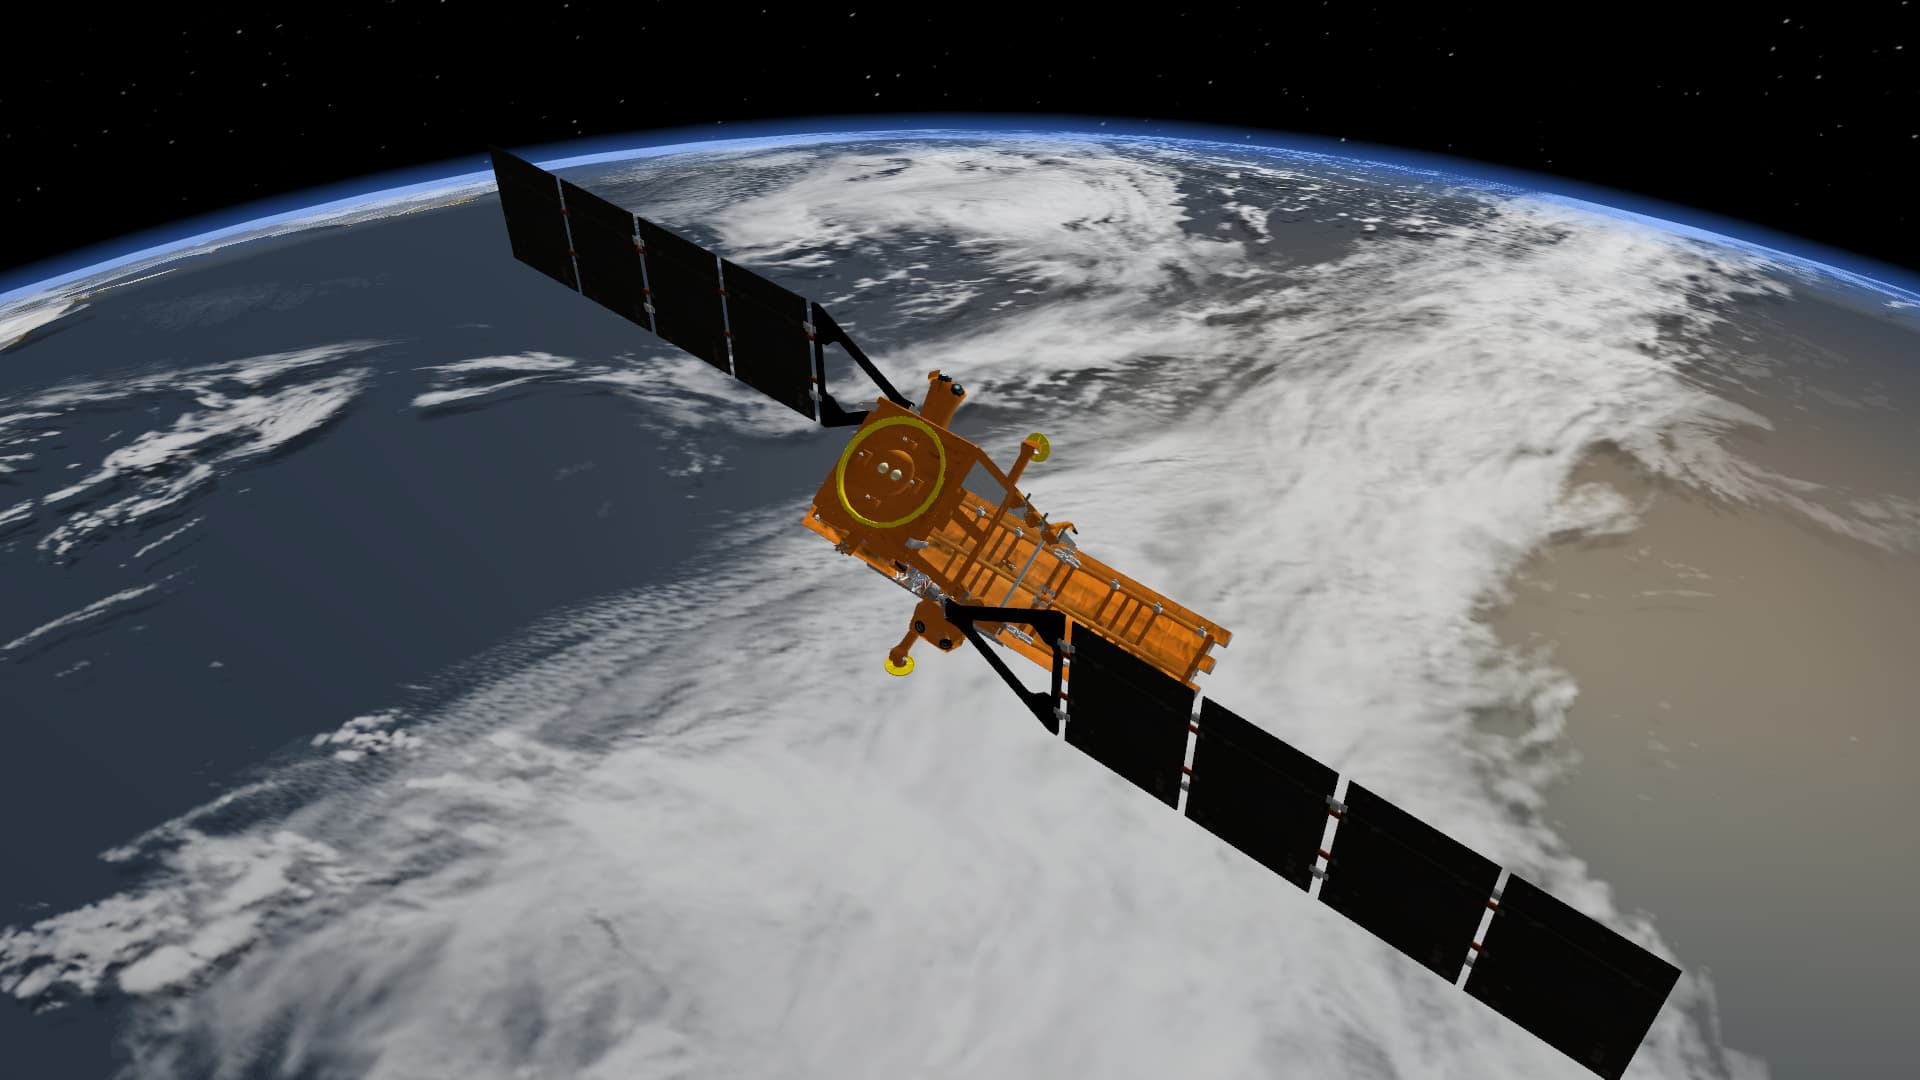
\includegraphics[width=0.9\textwidth,height=2.8cm]{cosmo.jpg}
        %\caption{Caption}
        %\label{fig:enter-label}
    \end{figure}
\column{0.5\textwidth}

    \begin{figure}
        \centering
        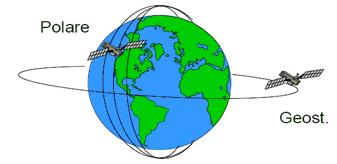
\includegraphics[width=0.9\textwidth]{orbita.jpg}
        %\caption{Caption}
        %\label{fig:enter-label}
    \end{figure}


    
\end{columns}



\end{frame}


\begin{frame}{Specifiche Satellite}

\begin{block}{Sensore SAR}

    \begin{itemize}
        \item Risoluzione spettrale: banda X (tra $2.8cm $ e $3.4 cm$ di lunghezza d'onda).
        \item Risoluzione spaziale: molto elevata, da $0,3m$ (in modalità Spotlight) a $10m$ (altre modalità).
        \item Risoluzione radiometrica: $10$ bit.    
        \item Capacità di operare in qualsiasi condizione atmosferica.
    \end{itemize}
        
    \end{block}

    \begin{figure}
        \centering
        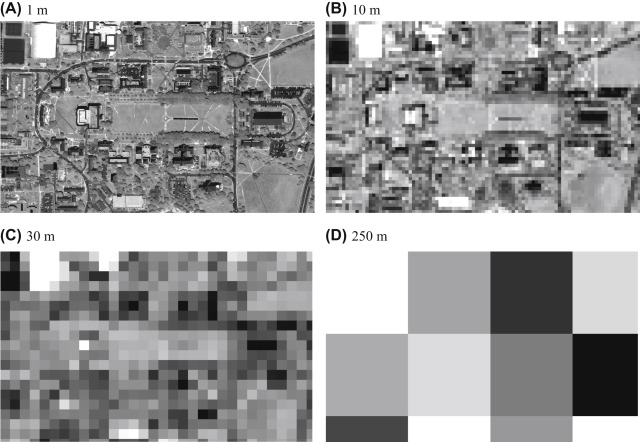
\includegraphics[width=0.45\textwidth,height=3.2cm]{risspaz.jpg}
        %\caption{Caption}
        %\label{fig:enter-label}
    \end{figure}
    
\end{frame}

\begin{frame}{Payload addizionali}

    
\begin{columns}
\column{0.02\textwidth}
    \column{0.5\textwidth}
    
            \begin{block}{Preprocessing on-board}      
            Attraverso un chip a basso consumo energetico è possibile elaborare l'immagine on-board applicando modelli di machine learning e sfruttare algoritmi di percorso ottimo per indicare percorsi sicuri e allarmare circa situazioni emergenziali. Ciò permette di velocizzare e ottimizzare la trasmissione dati anche attraverso l'implementazione di parallelismi nel calcolo e multiplexing nella trasmissione.         
            \end{block}
    
        \column{0.48\textwidth}   
            \begin{figure}
                \centering
                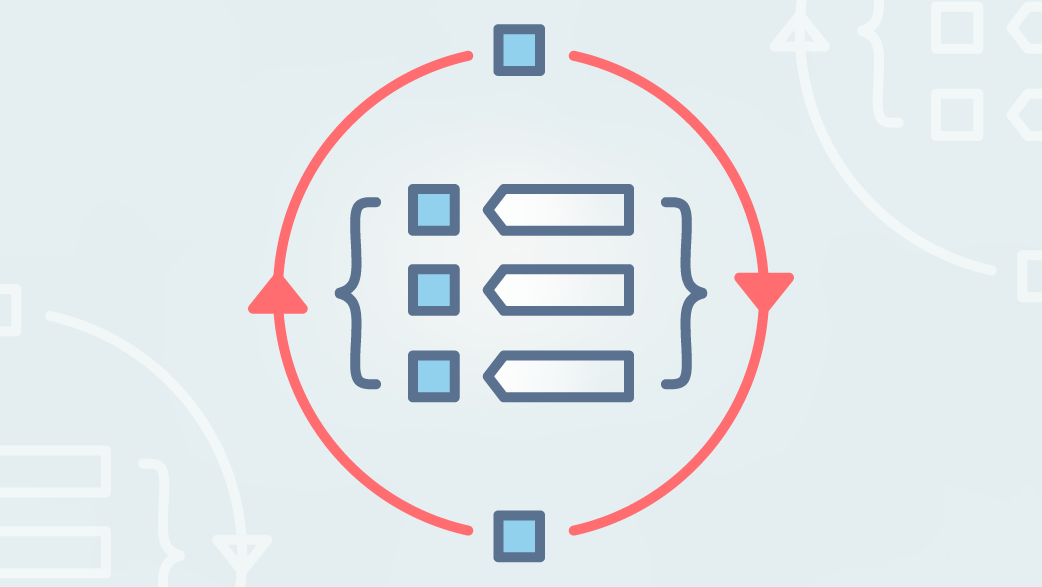
\includegraphics[width=0.8\textwidth]{proc.png}
                %\caption{Caption}
                %\label{fig:enter-label}
            \end{figure}    
            \begin{figure}
                \centering
                
\includegraphics[width=0.8\textwidth]{ai.jpg}
                %\caption{Caption}
                %\label{fig:enter-label}
            \end{figure}    
    \end{columns}
    
\end{frame}

\begin{frame}{Ground Segment}
\begin{columns}
\column{0.02\textwidth}
        \column{0.5\textwidth}
            \begin{block}{}
            \begin{itemize}
                \item \textbf{Facilities per il lancio}: lanciatore Vega-C, che sarà utilizzato per i prossimi due lanci dei satelliti COSMO-SkyMed.
                \item \textbf{Pianificazione acquisizione}: programmazione di tempi e modi di acquisizione delle immagini.
                \item \textbf{Ricezione e trasmissione dati}: due stazioni di terra con antenne per scaricare i dati e comunicare con il satellite.
            \end{itemize}
            \end{block}
            
        \column{0.48\textwidth}       
            \begin{figure}
                \centering
                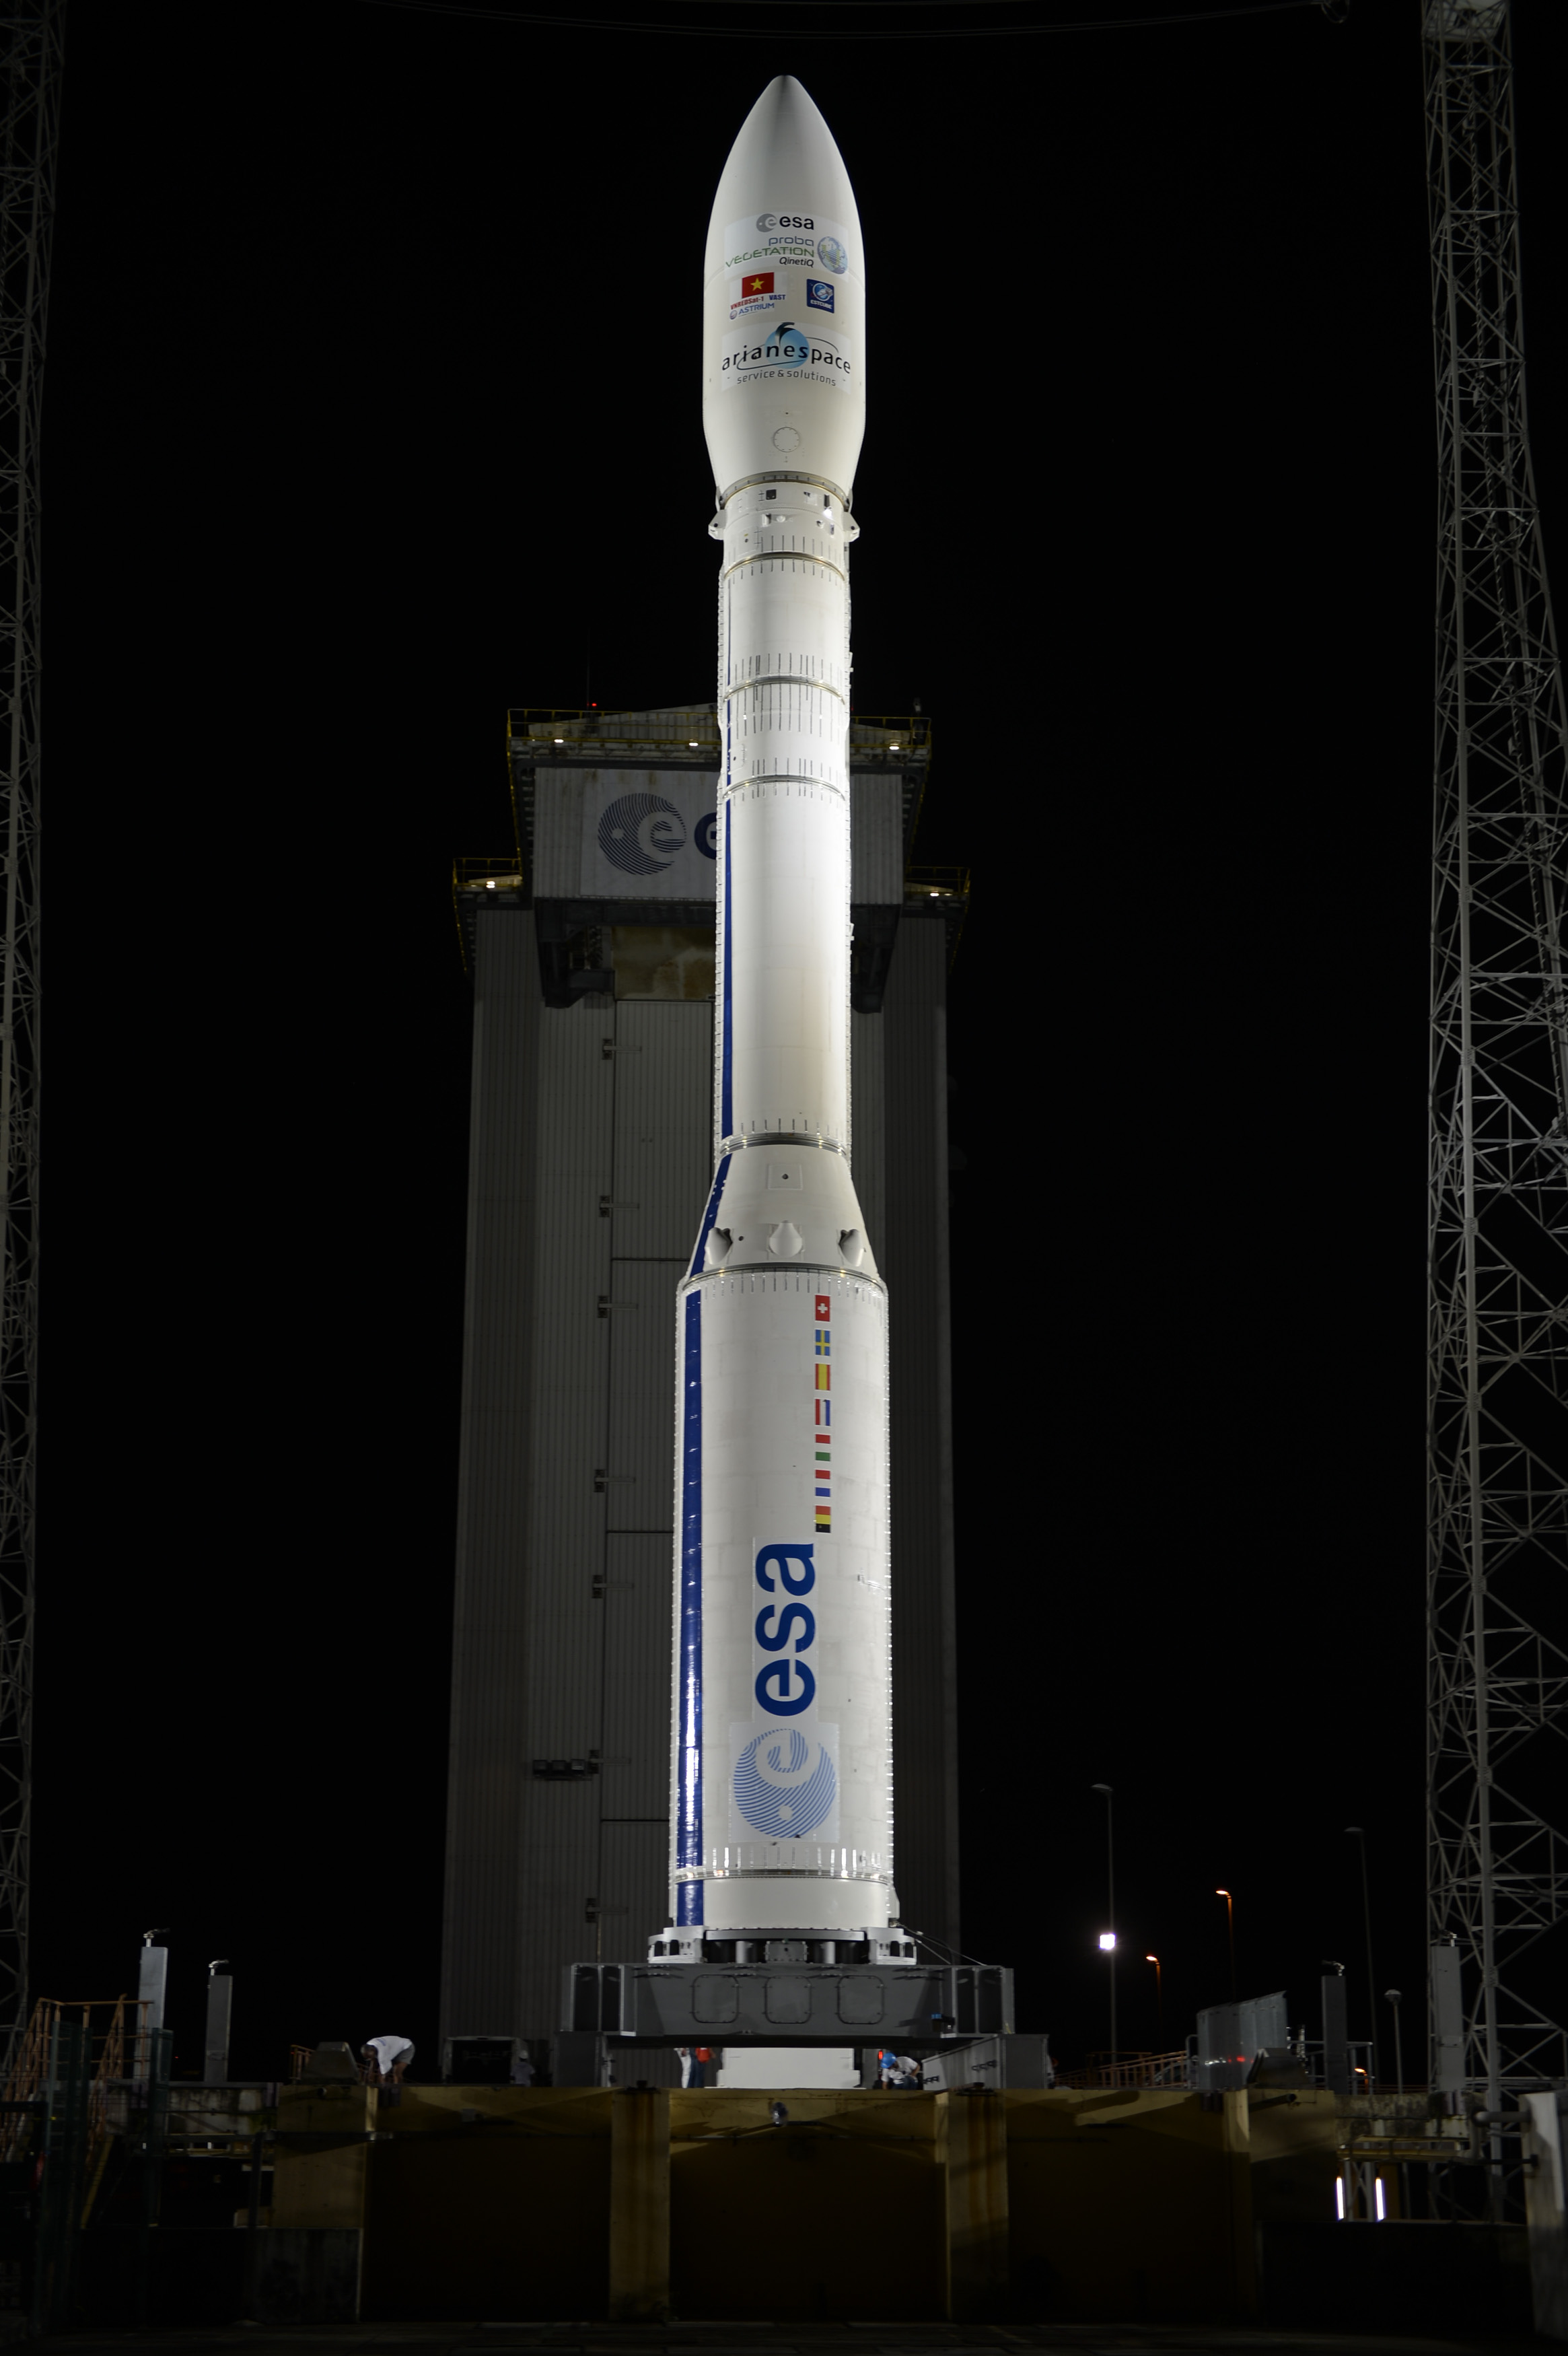
\includegraphics[height=6cm]{vega.jpg}
                %\caption{Caption}
                %\label{fig:enter-label}
            \end{figure}
 \end{columns}

\end{frame}

\begin{frame}{Costi}

\begin{center}
\begin{tabular}{|c|c|c|}
%\cline{2-4}
\hline
& \textbf{Modello} & \textbf{Costo}\\
%\cline{2-4}
\hline
\multicolumn{1}{ |c| }{\multirow{2}{*}{\textbf{Obiettivi}}}& 
  \multicolumn{1}{ c| }{Monitoraggio zone a rischio} & 3 \\
\cline{2-3}

\multicolumn{1}{ |c| }{} & \multicolumn{1}{ c| }{Miglioramento trasporto} & 
  3 \\
\hline

\textbf{Satellite} & Cosmo-Skymed & 12\\

\hline

\textbf{Payload} & Analisi dati on-board & 6\\



\hline

\multicolumn{1}{ |c| }{\multirow{3}{*}{\textbf{Infrastrutture}}}& 
  \multicolumn{1}{ c| }{Facilities per il lancio} & 4 \\
  
\cline{2-3}

\multicolumn{1}{ |c| }{} & \multicolumn{1}{ c| }{Pianificazione acquisizioni} & 
  2 \\

\cline{2-3}

\multicolumn{1}{ |c| }{} & \multicolumn{1}{ c| }{Ricezione e Trasmissione dati} & 
  5 \\

\cline{2-3}

\multicolumn{1}{ |c| }{} & \multicolumn{1}{ c| }{2 Antenne} & 
  4 \\

\hline

\multicolumn{1}{ |c| }{\multirow{2}{*}{\textbf{Lanciatore}}}& 
  \multicolumn{1}{ c| }{Vega-C} & 6  \\

\cline{2-3}

\multicolumn{1}{ |c| }{} & \multicolumn{1}{ c| }{Carburante} & 
  5 \\

\hline




\end{tabular}
\end{center}
    
\end{frame}



\begin{frame}{Business Model}

\begin{figure}
    \centering
    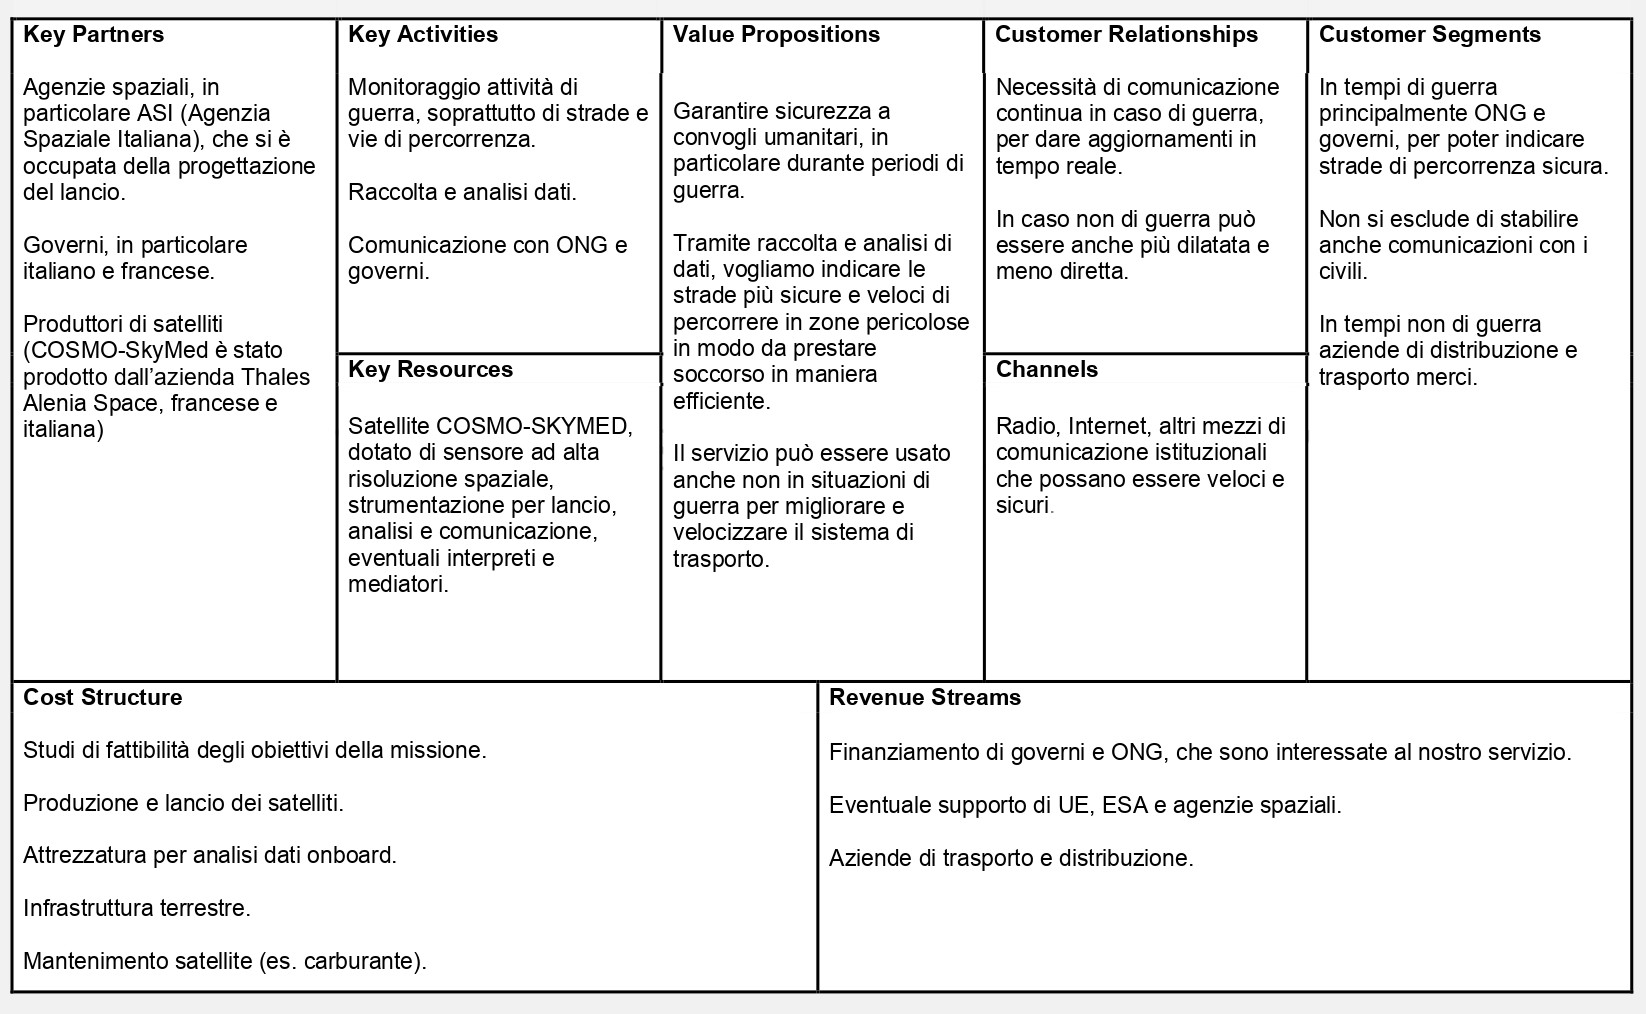
\includegraphics[width=\textwidth]{business-modeldausare.jpg}
    %\caption{Caption}
    %\label{fig:enter-label}
\end{figure}
    
\end{frame}

\begin{frame}{Valutazione Rischio}

\begin{figure}
   \centering
  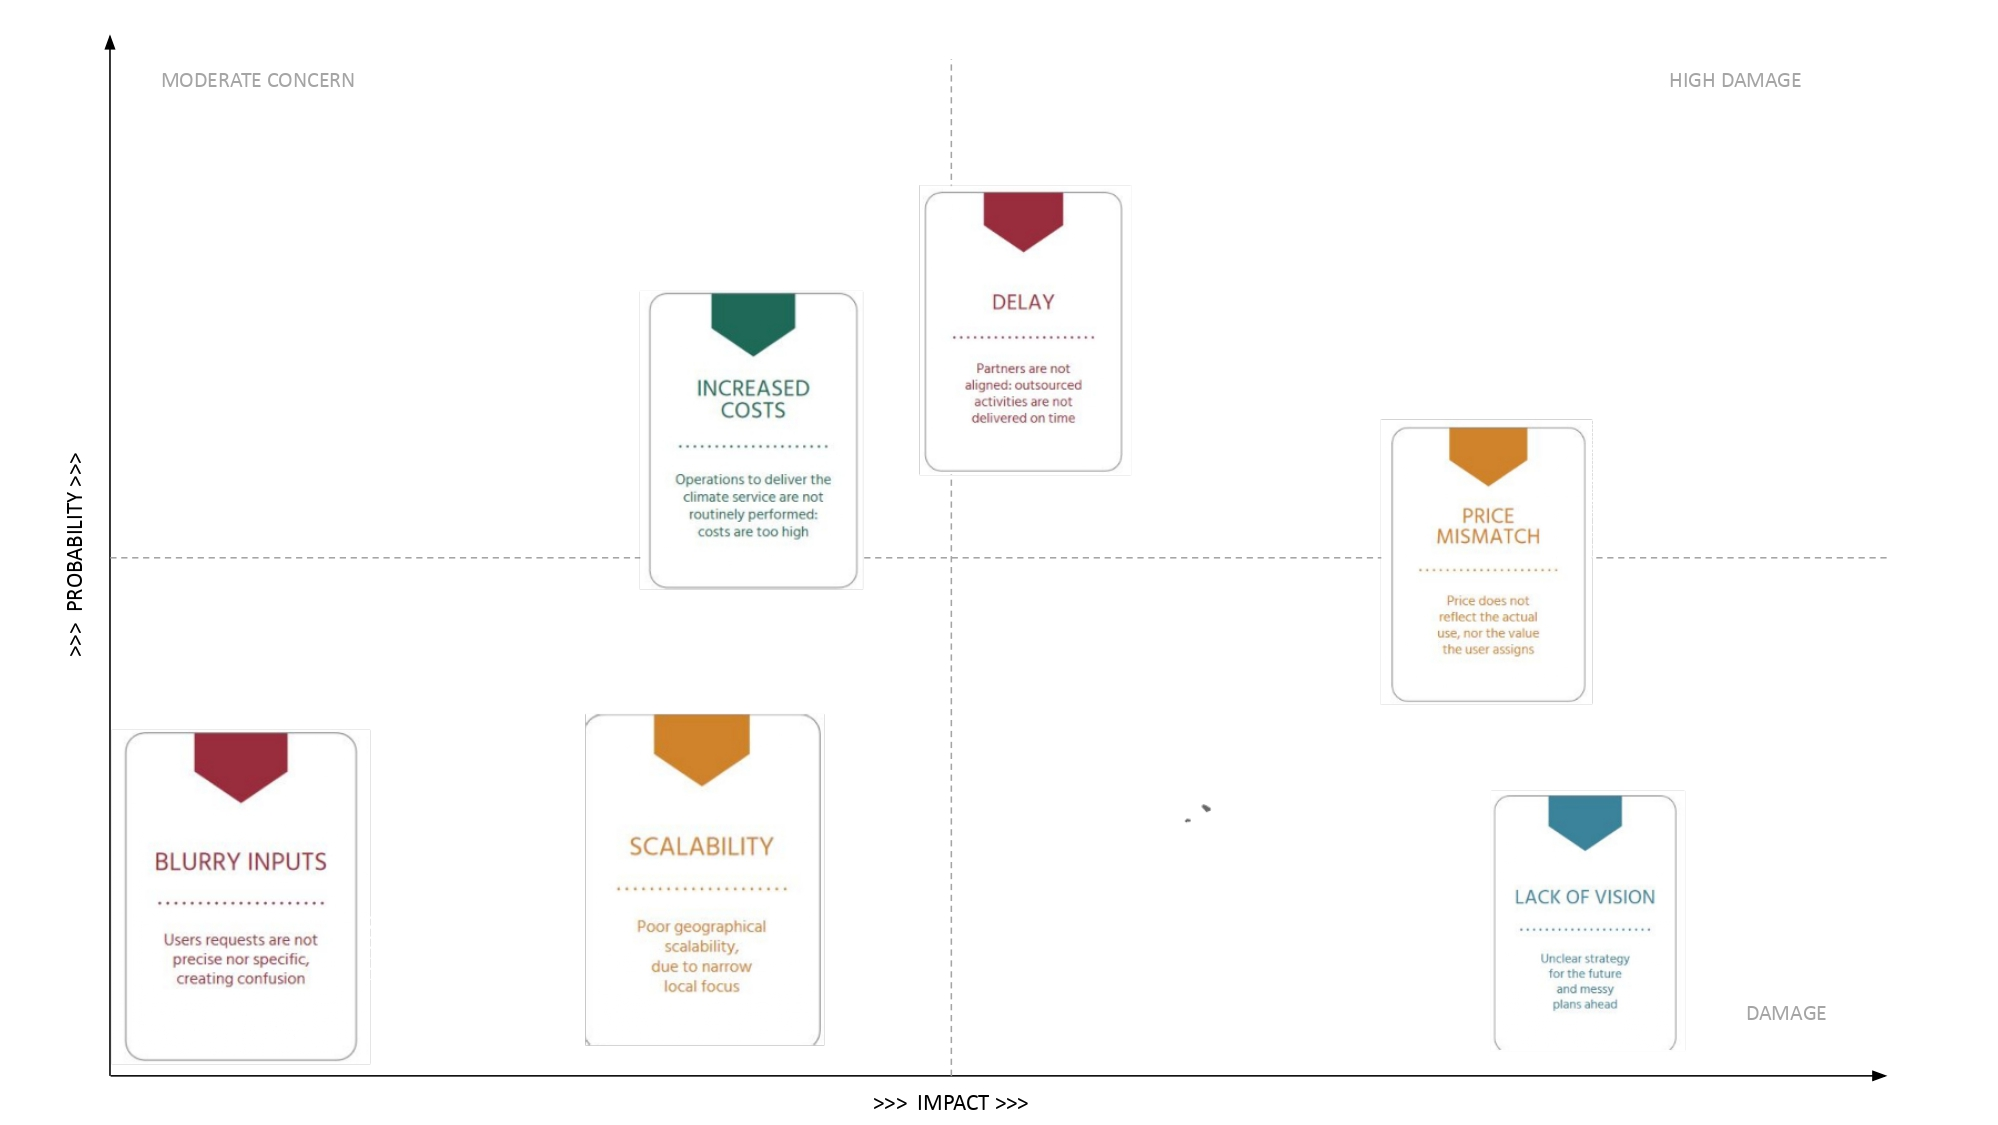
\includegraphics[width=\textwidth]{Riskdamettere.jpg}
    %\caption{Caption}
    %\label{fig:enter-label}
\end{figure}
    
\end{frame}

\begin{frame}{Bibliografia breve}

\begin{itemize}
    \item https://www.telespazio.com/it/business/space-programmes/cosmo-skymed
    \item https://earth.esa.int/eogateway/missions/cosmo-skymed
    \item https://www.asi.it/en/earth-science/cosmo-skymed/
\end{itemize}


    
\end{frame}






\end{document}
